\section{Fabrication}
\label{sec:Fabrication}
Three distinct fabrication techniques for soft actuators are show-cased with the help of the previously described multi-segment arm designs.
Table~\ref{tab:MachineTools} contains the superscript references to machine tools and materials used.

	
\subsection{Soft Lithography with Heterogenous Embeddings}
\label{subsec:Fabrication, Soft Lithography with Heterogenous Embeddings}
Soft lithography with heterogeneous embedding as a fabrication technique is shown for a ribbed actuator morphology. The ribbed manipulator is composed of six actuator segments and is fabricated from various soft and semi-soft materials.
Seven constraint supports (Fig.~\ref{fig:ribbed fab process}d) are 3D printed$^1$ and placed into a constraint layer mold (Fig.~\ref{fig:ribbed fab process}f), which is also 3D printed.
The constraint film (Fig.~\ref{fig:ribbed fab process}c) is cut from a thin acetal sheet$^8$ using a laser$^2$ and inserted through the aforementioned supports.
Above and below the constraint film, eight pieces of silicone tubing (Fig.~\ref{fig:ribbed fab process}a) are threaded through the supports.
Silicone rubber$^3$ is then mixed and poured into the constraint layer mold, immersing tubing, film, and supports in a layer of elastomer to create the composite constraint layer (Fig.~\ref{fig:ribbed fab process}g).
The uncured rubber inside the mold is then immediately degassed using a vacuum chamber$^4$.
Once cured, small holes are created in the constraint layer to pierce the embedded tubing at specific locations, allowing each line to independently address a group of fluidic channels.
Elastomer pieces containing channels (Fig.~\ref{fig:ribbed fab process}b) are casted and cured separately using a similar molding technique.
Those cured elastomer pieces (Fig.~\ref{fig:ribbed fab process}b) are then carefully attached to both faces of the constraint layer using a thin layer of silicone rubber.
Lastly, the printed feet (Fig.~\ref{fig:ribbed fab process}e) are attached to the constraint supports (Fig.~\ref{fig:ribbed fab process}d) to create an attachment point for ball transfers (Fig.~\ref{fig:ribbed_manipulator_design}d).
These mechanisms prevent the arm from tipping and help constrain the arm's motion to the X-Y plane.

\begin{figure}[htb]

\includegraphics[width=\columnwidth]{figures/fabrication/fab_ribbed_process.eps}
\caption[Fabrication process for a ribbed manipulator morphology]{Fabrication process for a ribbed manipulator morphology: silicone tubing (a), elastomer pieces containing channels (b), constraint film (c), constraint supports (d), feet (e), constraint layer mold (f), and composite constraint layer (g).}
\label{fig:ribbed fab process}
\end{figure}

\subsection{Retractable Pin Casting}
\label{subsec:Fabrication, Retractable Pin Casting}
The cylindrical manipulator is fabricated through a casting process that uses pourable silicone rubber$^{3,5}$ and 3D printed molds$^1$.
Figure~\ref{fig:cylindrical_fab} details this process.

First, each body segment is independently fabricated in steps 1-3 and later these segments are joined serially to form the arm in steps 4 and 5.
To start, a four piece mold is printed.
The mold is then poured in two steps.
In step 1, a low elastic modulus rubber$^3$ is mixed, degassed in a vacuum$^4$, and poured to form the body segment's soft outer layer shown in \emph{white}.
The mold's outer piece, one half of it is shown in \emph{green}, functions to form the segment's exterior.
Metal rods shown in \emph{pink} are inserted into the mold and are held in place by the \emph{orange} bottom piece of the mold.
These rods will form the cavities for the segment's two lateral fluidic actuation channels.

After the outer layer has cured, the \emph{red} rigid sleeve is removed in step 2 from the extruded feature of the \emph{orange} bottom piece of the mold.
This produces a cavity into which a slightly stiffer rubber$^5$ is poured, forming the segment's partially constraining inner layer shown in \emph{cyan}.
The extruded feature of the \emph{orange} bottom piece, shown by its \emph{orange} end tip, functions to produce the segment's hollow interior core.
In step 3, the body segments are removed from their molds and joined to rubber$^5$ endplates shown in \emph{cyan} using silicone adhesive$^6$.
The small \emph{yellow} channel inlets were added on one side of the \emph{pink} metal pins during step 1.
In step 4, soft silicone tubes$^7$ are joined to each embedded channel's inlet.
The resulting bundle of tubes is passed through each segment's hollow interior.
Lastly, in step 5 multiple body segments are attached at their endplates using the same adhesive$^6$.

\begin{figure}[htb]
\centering
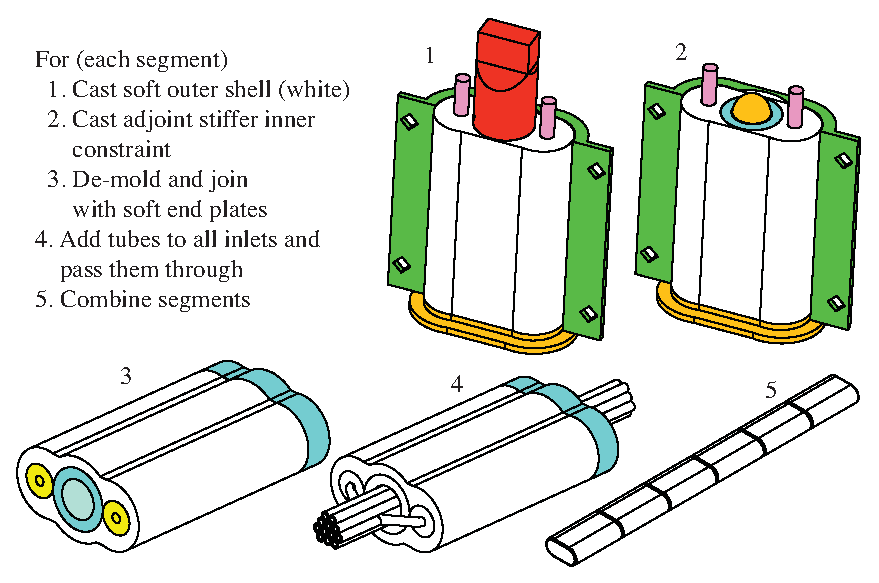
\includegraphics[width=\columnwidth]{figures/fabrication/fab_cylindrical_process.eps}
\caption[Fabrication process for the cylindrical manipulator morphology]{Fabrication process for the cylindrical manipulator morphology: Each body segment is casted using a two step process where the outer soft layer (\textbf{1}) and inner stiffer layer (\textbf{2}) are poured. Once cured, the segments are joined to endplates using silicone adhesive (\textbf{3}). Next, silicone tubing is connected to each embedded channel and the resulting tubing bundle is run inside each segment's hollow interior (\textbf{4}). Lastly, the body segments are serially connected using adhesive to form the manipulator (\textbf{5}).}
\label{fig:cylindrical_fab}
\end{figure}

\subsection{Lost Wax Casting}
\label{subsec:Fabrication, Lost Wax Casting}
Existing soft manipulators are produced through a multi-step lamination process, which produces seams and is easy to delaminate.
This limits their range of applications and lifetime.
By abandoning the need for a lamination process, arbitrary shaped internal channels can be achieved to enable a wider range of applications.
For these reasons, we introduce lost-wax casting as part of the fabrication process for soft actuators.
%The actuated cavities of the soft actuator are achieved by using bees-wax core$^{8}$, pourable silicone rubber$^{2,4,7}$ and 3D printed molds$^1$.
As an example, we fabricate the pleated actuated using the lost-wax approach.
The complete fabrication process for the pleated manipulator consists of eight steps that are depicted in Figure~\ref{fig:pleated_fab} and a final concatenation step.

\begin{figure}[htb]
\centering
   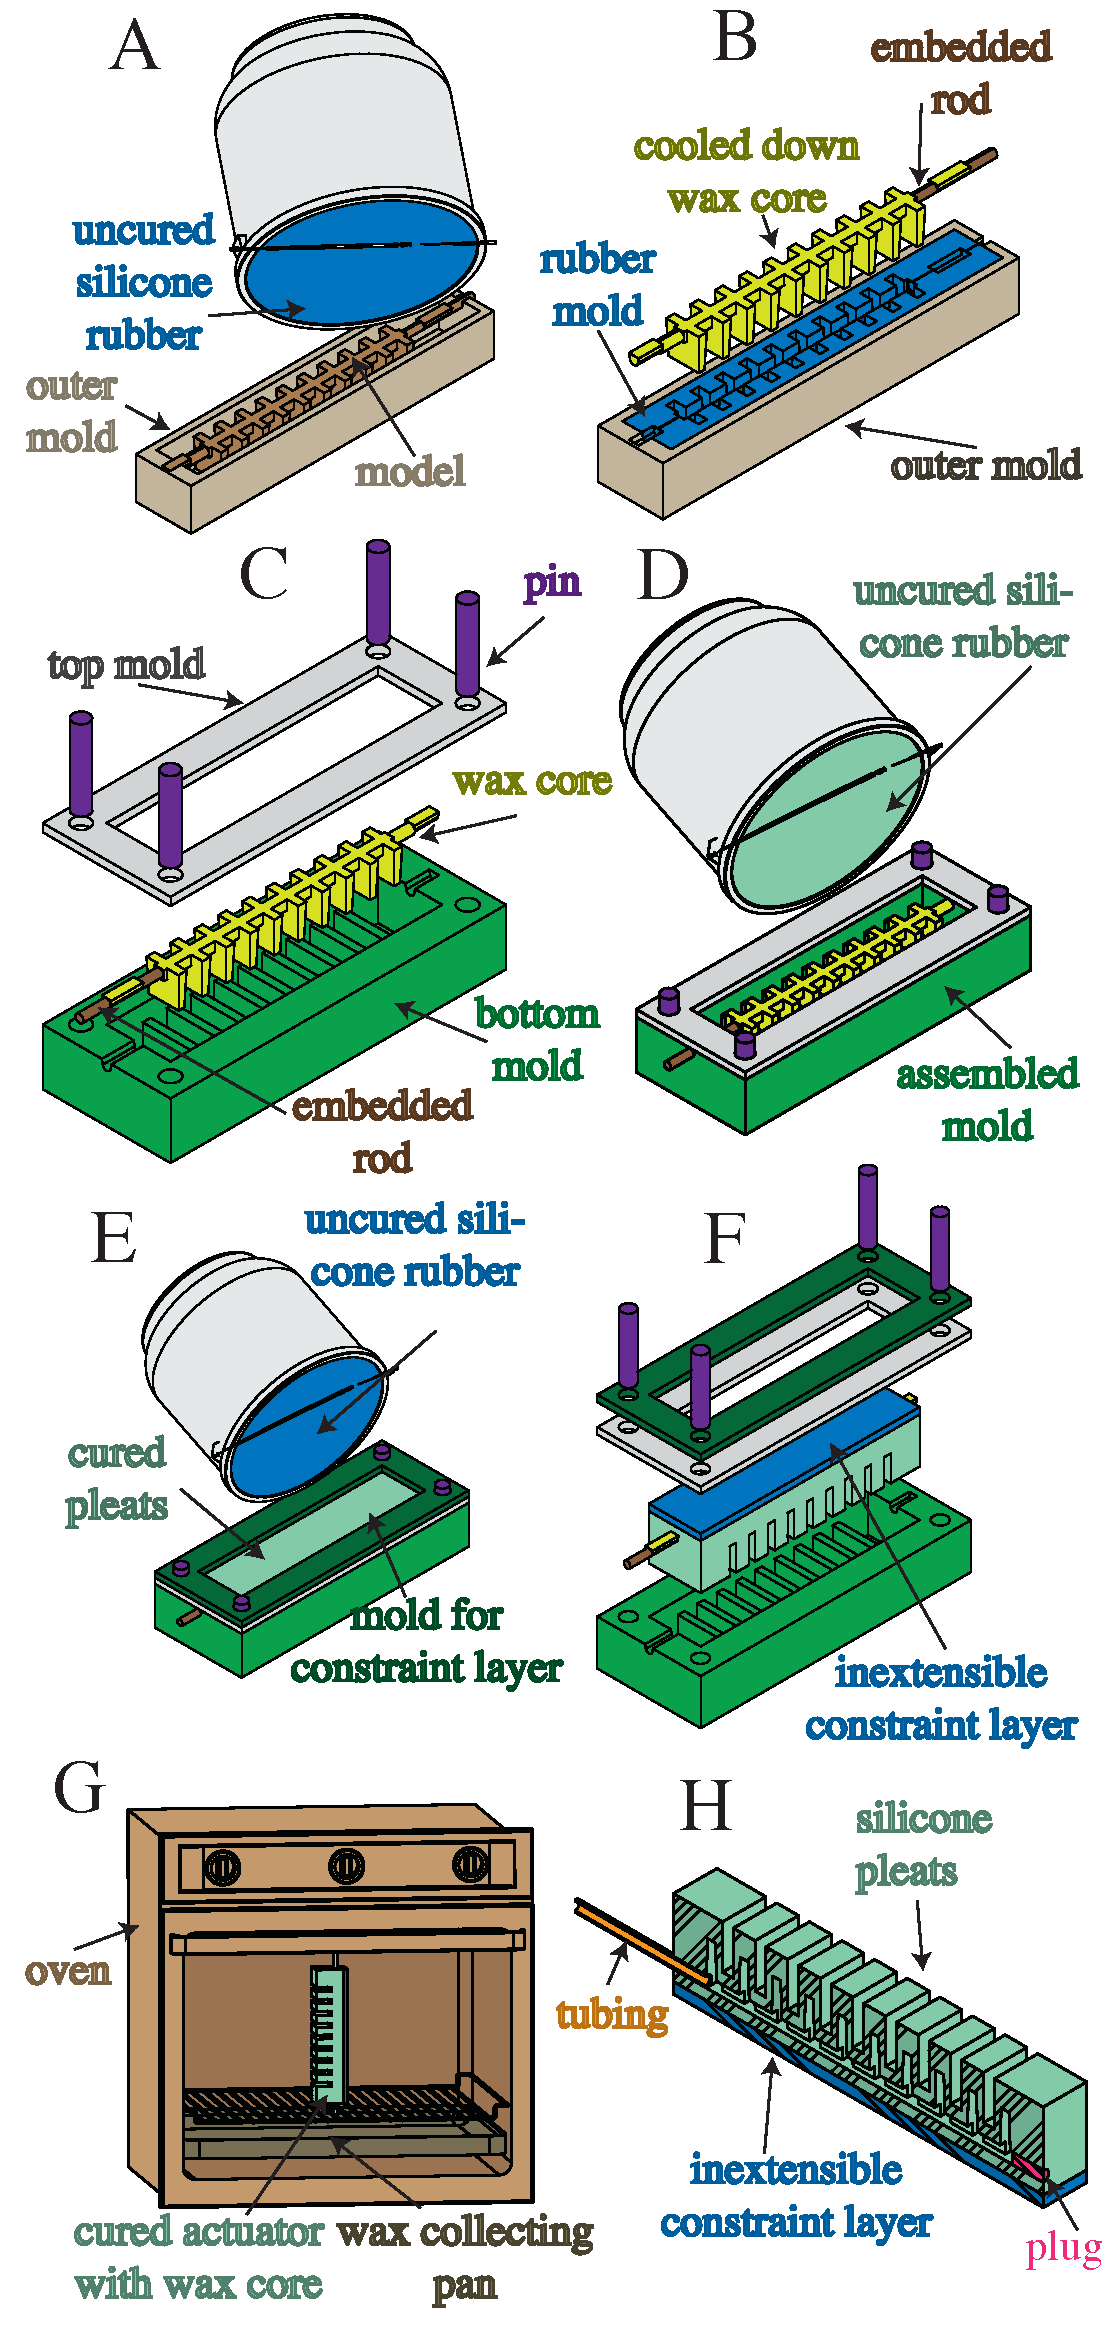
\includegraphics[width=\columnwidth]{figures/fabrication/fab_pleated_process.pdf}
      \caption[Fabrication process for the pleated actuator morphology]{Fabrication process for the pleated actuator morphology: (\textbf{A}) Pour and cure a rubber mold, (\textbf{B}) pour wax core with embedded supportive rod, (\textbf{C}) combine bottom mold, top mold and wax core using pins, (\textbf{D}) pour rubber into assembled mold, (\textbf{E}) pour stiffer rubber on top of the cured actuator to form a constraint layer, (\textbf{F}) remove cured actuator from mold, (\textbf{G}) melt out wax core from the actuator using an oven, and (\textbf{H}) add silicone tubing and plug using silicone sealant.}
      \label{fig:pleated_fab}
\end{figure}

In step (A), harder silicone rubber$^{10}$ is poured into a mold, which contains a 3D printed model of the wax core.
In preparation for step (B), the model is removed and the rubber mold is left inside the outer mold.
Next, a rigid rod or tube, for example made of carbon fiber$^{12}$, is used as a supportive inlay for the wax core.
The rod is laid into the cavity of the rubber mold, supported on both ends by the outer mold.
This ensures that the wax core does not break when removed from the rubber mold.
Mold release spray is applied to the silicone rubber mold to ease the wax core removal process.
The wax$^{11}$ is heated up until it becomes fully liquefied.
The assembly of the rubber mold and the outer mold is heated up for a few minutes to the same temperature as the wax.
Using a syringe, the liquid wax is injected into the assembly.
Within a few minutes, the injected wax will start to solidify and significantly shrink in volume; this is counteracted by injecting more hot wax into the solidifying wax core during the cool down period.
In step (B), the wax core is first allowed to completely cool down, then it is released from the mold.
In step (C), the cooled down wax core is assembled together with the bottom mold, which defines the pleated structure of the actuator.
The mold assembly is aligned with a top mold using pins. This top mold provides additional volume to cover the wax core.
In step (D), low elastic modulus rubber$^3$ is mixed, degassed in a vacuum$^4$, and poured to form the pleats and allowed to cure.
In step (E), stiffer rubber is poured on top of the cured pleats to form a constraint layer.
In step (F), the cured actuator is removed from the mold.
In step (G), most of the wax core is melted out by placing the cured actuator into an oven in an upright position.
After this, remaining wax residues are cooked out in a boiling water bath.
Finally, in step (H) a silicone tube$^9$ and a piece of silicone cord$^13$ get covered with silicone adhesive$^6$ and are inserted into the front and back holes, respectively.

Lastly, the actuator can be used as a unidirectional gripper or as one agonist side segment of a multiple body manipulator, where each segment can be actuated bidirectionally; see Section~\ref{subsec:Manipulators, Pleated}.

\begin{table}[htb]
\caption{Commercially Available Tools and Equipment}
\centering
\begin{tabular}{c l l}
\hline
\hline
\# & Product Name & Company\\
\hline
1 & Fortus 400mc & Stratasys\\
2 & VLS3.50 & Universal Laser Systems\\
3 & Ecoflex 0030 & Smooth-On\\
4 & AL Cube & Abbess Instr. \& Systems\\
5 & Mold Star 15 & Smooth-On\\
6 & Silicone Sealant 732 & Dow Corning\\
7 & PN 51845K52 & McMaster\\
8 & PN 5742T51 & McMaster\\
9 & PN 51845K53 & McMaster\\
10 & Mold Star 30 & Smooth-On\\
11 & Beeswax & Jacquard\\
12 & PN 2153T31& McMaster\\
13 & PN 9808K21& McMaster\\
\hline
\end{tabular}
\label{tab:MachineTools}
\end{table} 